\documentclass[11pt]{article}

\usepackage{geometry}
\usepackage{graphicx}
\usepackage{booktabs}
\usepackage{amsmath}

\geometry{margin=1in}

\title{QDK-010A: Noise-Response Statistical Reporting}
\author{Tai D. Nguyen}
\date{\today}

\begin{document}

\maketitle

\begin{abstract}
This report analyzes the QDK noise-response trajectories generated
under the reference stochastic model. The objective is to quantify
whether different encoded information structures produce separable
noise-response signatures.
\end{abstract}

\section{Objective}

QDK-010A evaluates the statistical separation of the three reference
structures:

\begin{itemize}
\item STRUCTURED
\item WEAK
\item ASYMMETRIC
\end{itemize}

The experiment is a numerical validation stage and does not constitute
validation on physical quantum hardware.

\section{Between-Structure Separation}

\begin{table}[h]
\centering
\begin{tabular}{lr}
\toprule
Comparison & Distance \\
\midrule
STRUCTURED\_vs\_WEAK & 1.835294 \\
STRUCTURED\_vs\_ASYMMETRIC & 1.043235 \\
WEAK\_vs\_ASYMMETRIC & 0.792065 \\
\bottomrule
\end{tabular}
\caption{Pairwise trajectory distances.}
\end{table}

\section{Separation Ratio}

The observed minimum between-structure distance is

\[
D_{\min} = 0.792065.
\]

The maximum mean within-structure variation is

\[
V_{\max} = 0.028152.
\]

The resulting descriptive separation ratio is

\[
R = \frac{D_{\min}}{V_{\max}}
  = 28.135090.
\]

This ratio is a descriptive metric. It is not a p-value, confidence
interval, or standardized statistical effect size.

\section{Interpretation}

The numerical experiment shows that the three encoded structures
produce distinguishable trajectories under the specified reference
noise model.

The result supports the hypothesis that the simulated noise response
can retain information about the encoded structure.

However, this result alone does not establish that physical quantum
noise universally acts as an information channel. Hardware-level
validation remains necessary.

\section{Reproducibility}

The analysis is derived from the QDK-009 result artifact:

\begin{verbatim}
results/qdk_009/QDK-009-STATISTICAL-VALIDATION.json
\end{verbatim}

\begin{figure}[h]
\centering
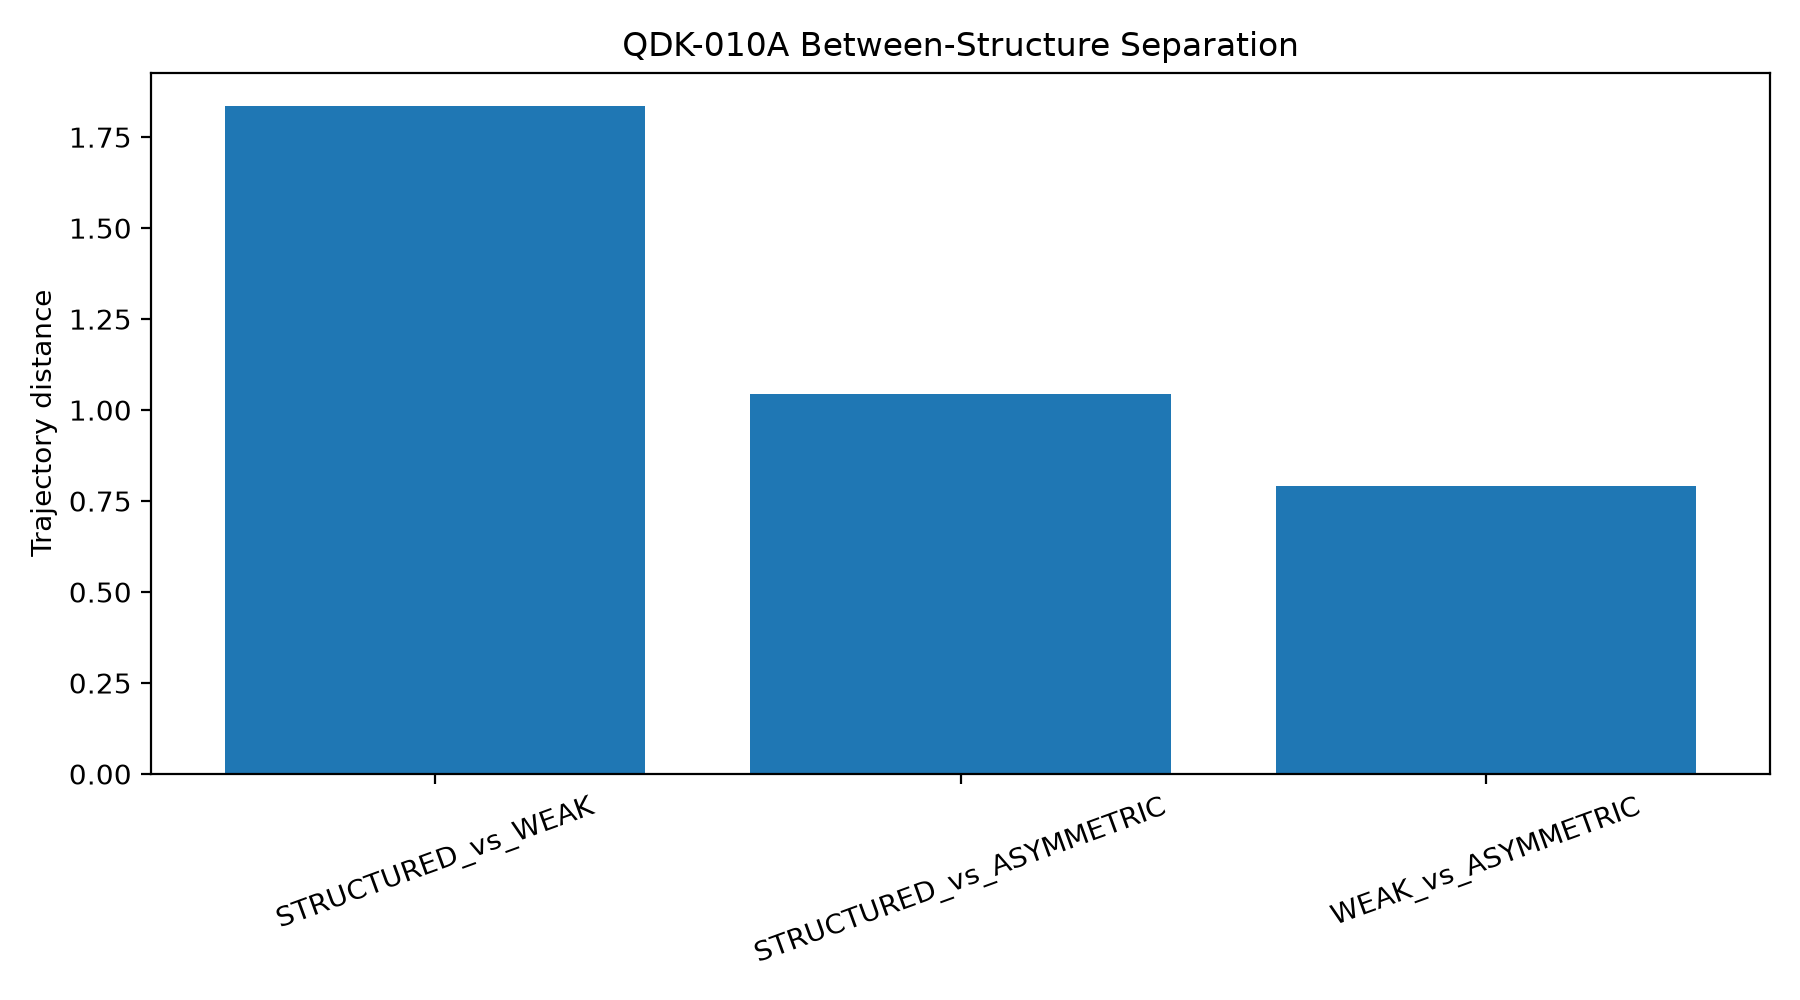
\includegraphics[width=0.9\textwidth]{../../results/qdk_010a/QDK-010A-between-distance.png}
\caption{Between-structure trajectory separation.}
\end{figure}

\begin{figure}[h]
\centering
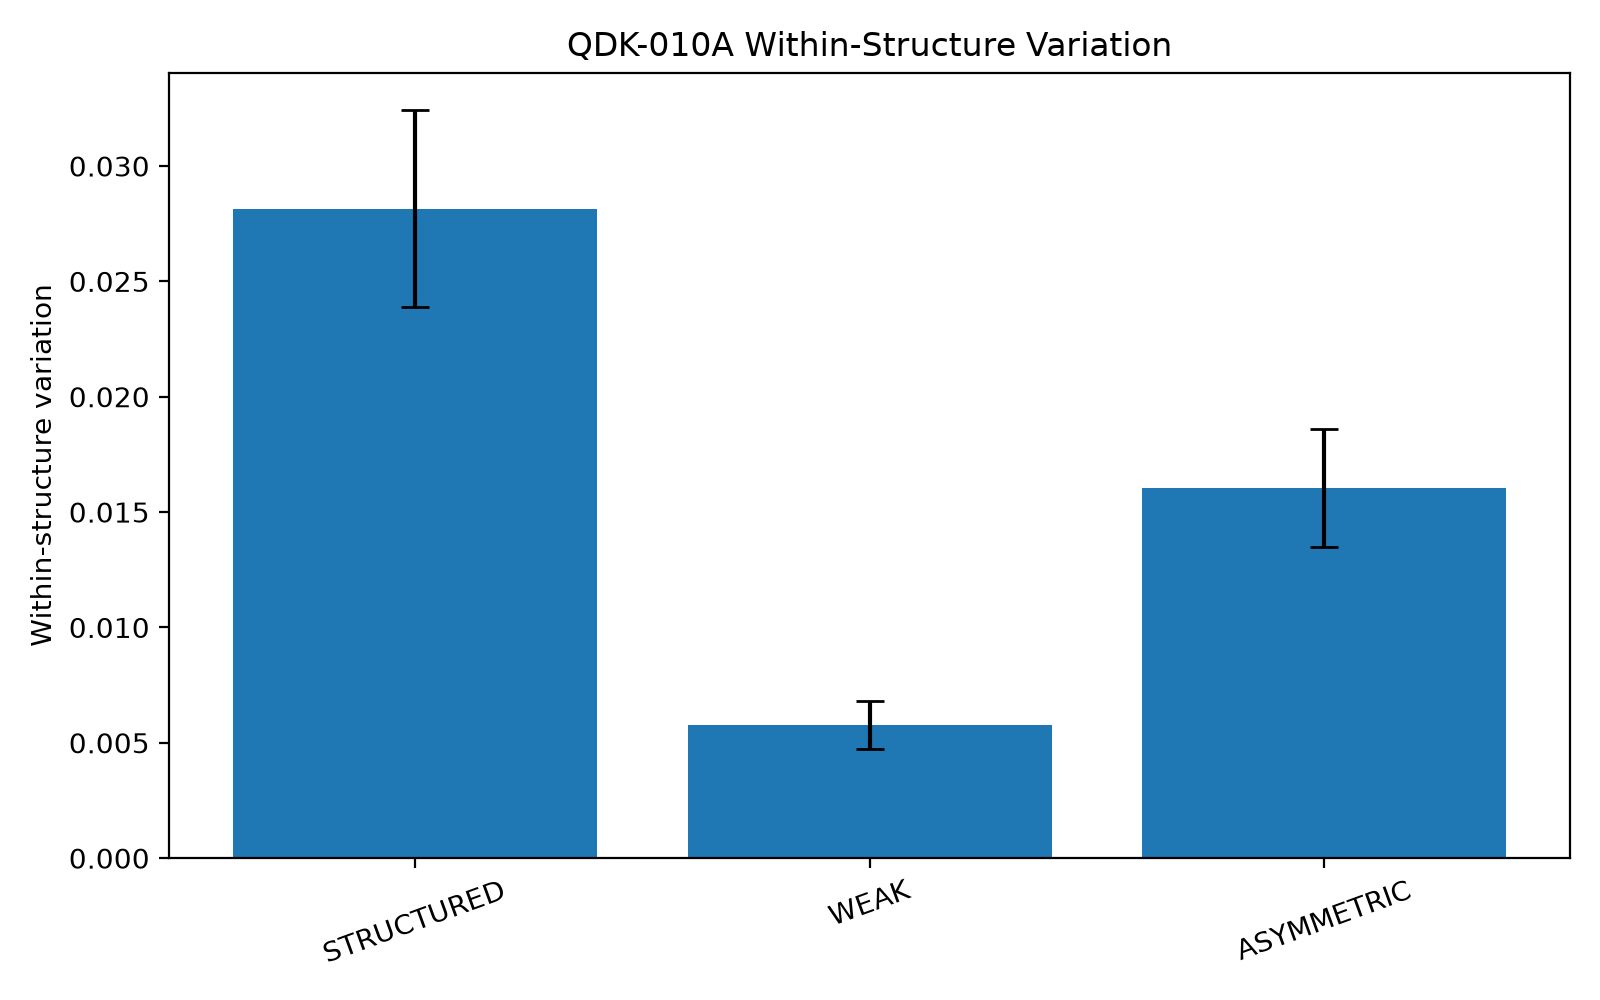
\includegraphics[width=0.85\textwidth]{../../results/qdk_010a/QDK-010A-within-variation.png}
\caption{Within-structure stochastic variation.}
\end{figure}

\section{Conclusion}

QDK-010A provides an automated statistical reporting layer for the
QDK noise-as-information research program.

The evidence is currently computational and model-dependent.
The next validation stage is QDK-010 hardware execution followed by
the same analysis pipeline.

\end{document}
